\paragraph{Generative Adversarial Imitation Learning (GAIL)} \mbox{} \\
\label{para:gail}
Generative Adversarial Imitation Learning was proposed for the first time in \cite{ho2016gail}, with the idea to improve the IRL setting, which is expensive to run, because of the double-nested optimization procedure. The authors in \cite{ho2016gail}, starting from a general Max-Ent formulation (Formula \ref{formula:regularized_max_ent}), obtained a characterization of the learned policy (Formula \ref{formula:policy_characterization}), where $\psi(c)$ is a cost-regularizer, $\psi^{*}(c)$ is its conjugate, and $\rho_{\pi}$ is the \textit{occupancy measure}, i.e., the distribution of state-action pairs that the agent encounters when navigating the environment with policy $\pi$. The interpretation of Formula \ref{formula:policy_characterization} is that the $\psi-regularized$ IRL finds a policy whose occupancy measure is similar to the expert's one, measured by $\psi^{*}$. The next-step was to choose an appropriate regularization function. In particular, by choosing the regularizer in Formula \ref{formula:ga_regularization}, the conjugate in Formula \ref{formula:ga_regularizer_conjugate} can be obtained, which is the classic Adversarial-Learning Loss, where the current policy $\pi^{L}$ plays the role of GAN generator, and $D$ is the GAN discriminator, which has to distinguish between state-action pairs generated either by the expert-policy or by the current policy.\begin{equation}
    \label{formula:regularized_max_ent}
    IRL_{\psi}(\pi^{E}) = \underset{c \in R^{S \times A}}{arg \ max} - \psi(c) +  (\underset{\pi^{L} \in \Pi}{\min} -\mathcal{H}(\pi^{L}) + \mathbb{E}_{\pi^{L}} \left [ c(s,a) \right ]) - \mathbb{E}_{\pi^{E}} \left [ c(s,a) \right ]
\end{equation}

\begin{equation}
    \label{formula:policy_characterization}
    RL \circ IRL_{\psi}(\pi^{E}) = \underset{\pi^{L} \in \Pi}{arg \ min}-\mathcal{H}(\pi^{L}) + \psi^{*}(\rho_{\pi^{L}} - \rho_{\pi^{E}}) 
\end{equation}

\begin{equation}
    \label{formula:ga_regularization}
    \psi_{GA}(c) = \left\{\begin{matrix}
        \mathbb{E}_{\pi^{E}}\left [ g(c(s,a)) \right ] &  if \ c < 0\\ 
        + \infty & otherwise
        \end{matrix}\right., \  g(x) = \left\{\begin{matrix}
                        -x - log(1- e^{x}) &  if \ c < 0\\ 
                        + \infty & otherwise
                        \end{matrix}\right.
\end{equation}

\begin{equation}
    \label{formula:ga_regularizer_conjugate}
    \psi^{*}_{GA}(\rho_{\pi^{L}} - \rho_{\pi^{E}}) = \underset{D\in(0,1)^{S \times A}}{max} \mathbb{E}_{\pi^{L}}\left [ \log(D(s,a))\right ] +\mathbb{E}_{\pi^{E}}\left [ \log(1 - D(s,a))\right ]
\end{equation}
Based on these considerations the Algorithm \ref{alg:gail} has been proposed. The algorithm comprises two fundamental steps, the first related to the Discriminator's parameter update and the second related to the policy's parameter update. Since GAIL has proven to be more effective than classic IRL algorithm \cite{ziebart2008maximum_entropy}, subsequent works have focused either on improving the sample efficiency, by replacing the model-free on-policy TRPO algorithm, with an off-policy RL algorithm, such as in \cite{kostrikov2018discriminator}, or by modifying the reward function in input to the RL algorithm \cite{fu2018airl,ghasemipour2020divergence_minimization_perspective}.\begin{algorithm}[tb]
\caption{Generative Adversarial Imitation Learning Algorithm}\label{alg:gail}
\begin{algorithmic}
\Require Expert Trajectories $\tau^{E} \sim \pi^{E}$, initial policy $\pi^{L}_{\theta}$, discriminator $D_{\omega}$
\For {$i=1, \dots, N$} 
    \State Sample trajectories, $\tau^{L}_{i} \sim \pi^{L}_{\theta}$
    \State Update Discriminator, $\mathbb{\hat{E}}_{\tau^{L}_{i}}\left [\nabla_{\omega} \log(D_{\omega}(s,a))\right ] +\mathbb{\hat{E}}_{\tau^{E}}\left [\nabla_{\omega} \log(1 - D_{\omega}(s,a))\right ]$
    \State Update Policy $\pi_{\theta}$, with TRPO \cite{schulman2015trpo}, and cost-function $C(s,a)=\log(D_{\omega}(s,a))$ 
\EndFor
\end{algorithmic}
\end{algorithm}All the cited methods have reported promising results on control tasks in a simulation environment \cite{brockman2016openai}, but they worked in a low-dimensional state-space, indeed when the GAIL method was adapted to work with a high-dimensional state-space, like in \cite{liu2018imitation_from_observation,reddy2019sqil,zolna2021task_relevant_ail,rafailov2021visual_ail}, it shown very poor results. In particular, with respect to the Adversarial Imitation Learning setting, works of interest are \cite{zolna2021task_relevant_ail,rafailov2021visual_ail}. In \cite{zolna2021task_relevant_ail}, the authors focused on solving the \textbf{casual-confusion} problem. This problem occurs when the discriminator, during the learning process, focuses on task-irrelevant features between expert and policy generated transitions, this causes the rewards to become uninformative. To reduce the casual-confusion problem, in \cite{zolna2021task_relevant_ail} two elements have been proposed: \begin{enumerate*}[label=(\textbf{\arabic*})]
    \item a regularization term, with the aim to make the discriminator \textbf{unable} to distinguish between constraining sets $I_{E}$ and $I_{A}$. The constraining sets are composed of expert and agent observations, such that a sample can belong either to $I_{E}$ or $I_{A}$, based on spurious features (e.g., a different gripper color);
    \item an early-stopping policy, Actor Early-Stopping (AES), that restarts the episode if the discriminator score at the current step exceeds the median score of the episode so far for $T_{patience}$ consecutive steps.
\end{enumerate*} The regularization term was defined as $\textit{accuracy}(\mathcal{I}_{E}, \mathcal{I}_{A}) = \frac{1}{2} \ \mathbb{E}_{s \in \mathcal{I}_{E}} \left[ \mathbf{1}_{D_{\omega} \geq  \frac{1}{2}}\right] + \frac{1}{2} \ \mathbb{E}_{s \in \mathcal{I}_{A}} \left[ \mathbf{1}_{D_{\omega} <  \frac{1}{2}}\right]$. In the end, the discriminator parameters were the result of $\underset{\omega}{max} \ G_{\omega}(s_{E},s_{A}) - \mathbf{1}_{\textit{accuracy}(\hat{s}_{E},\hat{s}_{A}) \geq \frac{1}{2}} G_{\omega}(\hat{s}_{E},\hat{s}_{A})$, where $G_{\omega}$ is the discriminator binary cross-entropy, $\hat{s}_{E} \in \mathcal{I}_{E}$, and $\hat{s}_{A} \in \mathcal{I}_{A}$. %The proposed system was tested on 4 tasks (Figure \ref{fig:trail}).
An agent was trained on each single task, according to the Distributed Distributional Deterministic Policy Gradients (D4PG) \cite{barth2018d4pg} RL algorithm, with reward-function $R(s_{t}) = - \log(1-D_{\omega}(s_{t}))$. Experimental results have shown how the proposed system overcomes the GAIL \cite{ho2016gail} baseline, both in setting with spurious features and without spurious features (Figure \ref{fig:trail_results}).\begin{figure}[tb!]
    \centering
    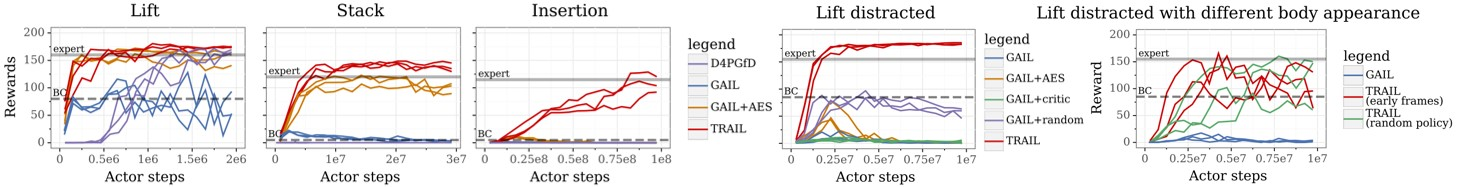
\includegraphics[width=\textwidth]{Figures/images/trail/trail_results.jpg}
    \caption{Experimental results on tasks without and with spurious features \cite{zolna2021task_relevant_ail}}    
   \label{fig:trail_results}
\end{figure}

\unskip The authors of \cite{rafailov2021visual_ail} made a step towards a more data efficient Adversarial Imitation Learning method. Indeed, they leveraged the idea of using a model-based approach in the context of high-dimensional state space. Still, instead of generating a dynamic model in the image space, the proposed method is based on encoding the observations defined in the image space into a corresponding latent space characterized by vectors of smaller dimension. Then subsequently go on to learn a dynamic model in that space. In this context the learning procedure is based on three main steps: \begin{enumerate*}[label=\textbf{(\arabic*)}]
    \item learn the \textit{Latent Dynamic Model}, $(\hat{\mathcal{U}}_{\beta},\hat{\mathcal{T}}_{\beta}, q_{beta})$, by maximizing the Expected Lower Bound (Formula \ref{formula:elbo}), where $\hat{\mathcal{U}}_{\beta}$ is the decoder, $q_{beta}$ is the encoder, and $\hat{\mathcal{T}}_{\beta}$ is the transition model;
    \item train a \textit{discriminator}, $D_{\theta}$, by minimizing the Adversarial Loss function (Formula \ref{formula:discriminator});
    \item train a \textit{policy} $\pi^{L}_{\theta}$, by maximizing the Value function (Formula \ref{formula:value_function}).
\end{enumerate*}
%\begin{algorithm}
    \caption{Variational Model-Based Adversarial Imitation Learning \cite{rafailov2021visual_ail}}
    \label{alg:vmail}
    \begin{algorithmic}
    \Require Expert Demonstrations $\mathcal{D}^{E}$, environment buffer $\mathcal{D}^{\pi^{L}}$
    \Require Policy $\pi^{L}_{\theta}$, discriminator $D_{\omega}$, variational model $(q_{\beta}, \hat{\mathcal{T}}_{\beta})$
    \For {$i=1, \dots, N$}
        \For {$t=1, \dots, T$}
            \Comment Data Collection
            \State Estimate latent state, $z_{t} \sim q_{\theta}(.|s_{t},z_{t-1},a_{t-1})$
            \State Sample action, $a_{t} \sim  \pi^{L}_{\theta}(a_{t}|z_{t})$
            \State Observ new state, $s_{t+1}$
        \EndFor
        \State Add transitions ${s_{1:T}, a_{1:T-1}}$ to $\mathcal{D}^{\pi^{L}}$
        \For {training iterations}
            \Comment Dynamic Learning
            \State Optimize Variational Model $(q_{\beta}, \hat{\mathcal{T}}_{\beta})$, Formula \ref{}
            \State Infer Expert Latent Space, $z_{1:T}^{E} \sim q_{\theta}(.| s_{1_T}^{E}, a_{1:T-1}^{E})$
            \State Generate latent rollouts, $z_{1:H}^{L} $ 
        \EndFor
    \EndFor
\end{algorithmic}
\end{algorithm}
\begin{equation}
    \label{formula:elbo}
    \underset{\beta}{max} \ \mathbb{E}_{q_{\beta}}\left[\sum_{t} \log(\mathcal{\hat{U}}_{\beta}(s_{t}|z_{t})) + \mathbb{D}_{KL}(q_{\beta}(z_{t}|s_{t},z_{t-1},a_{t-1})|| \mathcal{\hat{T}}_{\beta}(z_{t}|z_{t-1},a_{t-1})) \right]
\end{equation}

\begin{equation}
    \label{formula:discriminator}
    \underset{\theta}{min} \ \mathbb{E}_{(z,a) \sim \rho^{E}(z,a)} \left[-log(D_{\theta}(z,a))\right] + \mathbb{E}_{(z,a) \sim \rho^{\pi^{L}}_{\hat{\mathcal{T}}}} \left[-\log(1 - D_{\theta}(z,a))\right]
\end{equation}

\begin{equation}
    \label{formula:value_function}
    \underset{\pi^{L}_{\theta}}{max} \ V^{K}_{\theta,\beta}(z_{t}) = \underset{\pi^{L}_{\theta}}{max} \ \mathbb{E}_{\pi^{L}_{\theta}, \mathcal{\hat{T}}_{\beta}}\left[ \sum_{\tau = t}^{t+K-1} \gamma^{\tau-t} \log(D_{\theta}(z_{\tau}^{\pi^{L}_{\theta}}, a_{\tau}^{\pi^{L}_{\theta}})) + \gamma^{K}V_{\beta}(z_{t+K}^{\pi^{L}_{\theta}})\right]
\end{equation}
    
    
\noindent With this learning setting the proposed system outperforms previous works such as \cite{reddy2019sqil,kostrikov2018discriminator} both in terms of data-efficiency and overall performance, on a set of control tasks (Figure \ref{fig:vmail}).Generally speaking, the Generative Adversarial Imitation Learning has shown very promising performance in simulated control tasks and simulated robot manipulation tasks, even in complex high-dimensional state-space. However, it is not so clear, how these methods could perform in real-world robotic manipulation tasks, in terms of data-efficiency, generalization capability, and safety during real-world interactions.
\begin{figure}[htb!]
    \centering
    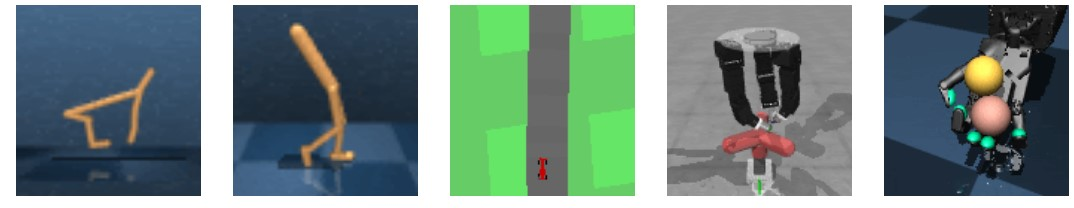
\includegraphics[width=0.75\textwidth]{Figures/images/vmail/control-tasks.jpg}
    \caption{Control tasks solved in \cite{rafailov2021visual_ail}. From left to right: cheetah run, walker walk, car racing, claw rotate, baoding balls}
    \label{fig:vmail}
\end{figure}
